\section{进程管理}
在正式介绍Linux内核中的进程和线程前,
我们先利用课程中了解到的进程和线程的概念尝试直接分析内核中进程的表示方式——进程控制块(PCB),
建立整体的认识.
最后,我们试着弄懂Linux的进程调度策略,并把重点放在最常用的
Completely Fair Scheduler(CFS)上.

\subsection{进程控制块}
\lstinline{struct task_struct} 是Linux内核的进程控制块(PCB).
它存储进程的标识符、进程的状态、指向存储进程上下文的数据结构的指针、调度所需的信息以及与进程相关的资源和指向其他 \lstinline{task_struct} 的指针等.
所有与进程有关的操作都会直接或间接地修改进程控制块来达到目的.
下面,我们介绍管理进程所需要的多种信息,并介绍它们是如何在 \lstinline{task_struct} 中表示的.

\begin{readsrcbox}{进程控制块}
	\lstinline{struct task_struct} 是在\lstinline{include/linux/sched.h}中定义的.
\end{readsrcbox}

\subsubsection{进程的状态} \label{process state}
首先是进程的状态,一个进程可能处于这些状态:
\begin{itemize}
	\item \lstinline{TASK_NEW}.
	      当一个进程刚创建时,它的状态就被设置为\lstinline{TASK_NEW},表示这个进程已经被创建,但是还没有开始运行.
	\item \lstinline{TASK_DEAD}.
	      进程已经结束.
	\item \lstinline{TASK_RUNNING}.
	      进程正在运行,即该进程在正在运行的进程的队列里.
	\item \lstinline{TASK_INTERRUPTIBLE} 或者 \lstinline{TASK_UNINTERRUPTIBLE}.
	      处于这两个状态的进程正在等待,但是只有 \lstinline{TASK_INTERRUPTIBLE} 状态的进程才会被信号唤醒.
	\item \lstinline{TASK_NOLOAD}.
	      类似 \lstinline{TASK_UNINTERUPTIBLE} 但是在统计数据中不被计入负载.
	      \footnote{见 \url{https://lore.kernel.org/lkml/alpine.LFD.2.11.1505112154420.1749@ja.home.ssi.bg/T/}}
	\item \lstinline{TASK_WAKING}.
	      进程已经被要求唤醒,但是还没有进入正在运行的进程队列.
	      \footnote{见 \url{https://lore.kernel.org/lkml/tip-e9c8431185d6c406887190519f6dbdd112641686@git.kernel.org/}}
	\item \lstinline{TASK_WAKEKILL}.
	      该进程收到SIGKILL信号时会被唤醒.
	\item \lstinline{TASK_TRACED}.
	      调试器暂停该进程来追踪它的运行状态.
\end{itemize}
这些状态被编码成掩码,读写进程的状态时,
需要用这些掩码操作 \lstinline{task_struct} 的 \lstinline{__state} 域.
比如识别一个进程是否处于某状态,
就要用它的 \lstinline{__state} 和 这个状态的掩码做与操作,
若结果为0则不处于这个状态.
这些状态中有的状态可以组合成新的掩码,方便使用.

\subsubsection{进程的CPU上下文} \label{context}
进程控制块还需要存储有关进程上下文的信息,例如有关栈和堆的信息和CPU内部寄存器的值.
这一部分信息既和内核的内存管理有关又依赖于具体的硬件架构,
是实现进程调度中挂起和重启进程所需要的数据结构.
\begin{readsrcbox}{架构相关代码}
	为了提高可移植性,Linux内核的代码区分不依赖于具体硬件架构的代码和针对特定架构的代码.
	架构相关的代码全部在 \lstinline{arch} 目录下.
	例如 x86和x86\_64的代码位于 \lstinline{arch/x86}.

	显然,所有的汇编代码都应该放在该目录.
	内存管理和进程管理所需的某些功能也依赖于CPU的特定功能,
	需要根据硬件功能定义数据结构和执行具体的指令,
	这些定义和实现也位于 \lstinline{arch} 下具体架构的目录下.
	不同的架构的代码尽量暴露出相同的接口,供架构无关代码使用.

	某一架构上的具体实现的文档可以在 \href{https://docs.kernel.org/arch.html}{\lstinline{Document/arch.rst}} 中的列表找到.
	例如\href{https://docs.kernel.org/x86/kernel-stacks.html}{\lstinline{Document/x86/kernel-stacks.rst}}介绍了x86\_64 CPU上内核为每一个进程维护的若干个栈.
\end{readsrcbox}
\lstinline{task_struct}的定义中,有一个 \lstinline{void *stack;} 域.
这不是该进程的用户态的栈的起始地址,
而是该进程的\textbf{内核栈}的起始地址,每次该进程通过系统调用从用户态进入内核态时,
内核中的代码都在这个内核栈上执行.

\lstinline{tast_struct}的最后一个成员是 \lstinline{struct thread_struct thread;},
进程在CPU上的运行状态存放在这个架构相关的结构体中.
x86\_64上该结构体的大小可以变化,因此它必须作为\lstinline{tast_struct}的最后一个成员.
这个 \lstinline{struct thread_struct} 的成员直接或间接地保存该进程的上下文.

我们在微机原理中学过x86\_32架构对于上下文切换有专门的硬件支持.
Global Descriptor Table(GDT)中有专门的描述符指向Task State Segment(TSS).
TSS可以用来存储所有的x86寄存器,
在需要时自动进行硬件上下文切换,把寄存器的值存储在旧的TSS中,然后把新TSS的内容加载到寄存器中.
x86\_64取消了硬件上下文切换的功能,但即使是在32位x86机器上,
Linux内核也不是用TSS来进行硬件切换,
因为考虑到其它架构几乎都不支持这一机制,使用软件实现上下文切换可移植性更好.

Linux 内核在上下文切换时,寄存器的值实际上是存在进程的内核栈上的.
进程在切换之前,一定正在该进程的内核栈上执行内核态的代码,
这时用户程序的寄存器已经在进入内核态后保存下来了,
要保存运行在内核态时的寄存器,只需要 \lstinline{pushq} 所有的\textit{被调用者保存}寄存器即可.
这是因为在进入当前栈帧前后,调用者一定已经保存了其所需的\textit{调用者保存}寄存器.
返回地址也在栈帧中有记录.
既然这个栈帧就记录着当前进程的上下文,PCB只需保存这个栈帧的地址即可.
因此 \lstinline{thread_struct} 有一个 \lstinline{unsigned long sp;} 域,
存放的就是切换前的寄存器sp的值,即这个栈帧的地址.

除了整数运算的寄存器,浮点和向量运算的寄存器也需要保存,
但是由于浮点和向量运算不像整数运算那样常见,
且保存这些状态有一定开销,
之前的Linux内核只在这些运算真正执行过时才保存对应的寄存器.
这种“懒惰”的保存方式是通过CPU的硬件支持完成的:
每次上下文切换时,CPU的TS标志位就被置为1;
每次浮点或向量运算指令执行时,若TS标志位为1,则会报“Device Not Available”异常.
内核在处理这个异常时会记录下来:该进程使用了浮点或向量运算.
再次切换进程时,若发现使用了浮点或向量运算,则保存相应的状态.\cite{bovet2005understanding}
而现代的CPU引入了特定的指令来保存FPU状态,
减小了保存FPU状态的开销,
而且程序越来越依赖向量指令来进行拷贝数据等操作,
所以Linux在2016年取消了“懒惰”的保存方式,
\footnote{见 \url{https://lore.kernel.org/lkml/e3b2baadcd19bf8abcd3bcd60d19e8e50e75f63a.1453510332.git.luto@kernel.org/}}
每次进程切换都保存FPU的状态.
除了进程切换,
另外一个需要保存和恢复FPU状态的时机是内核代码在用户上下文中使用浮点或向量运算的前后,
这也是按需进行的,
即返回用户态时,若改变了FPU状态才加载用户的FPU状态.

FPU的状态保存在 \lstinline{thread_struct} 的 \lstinline{struct fpu fpu;}域.
这个数据结构是变长的,这也是 \lstinline{struct thread_struct thread;}
要放在 \lstinline{task_struct} 最后的原因.

\begin{readsrcbox}{\lstinline{thread_struct}}
	\lstinline{thread_struct} 是架构相关的.
	x86的 \lstinline{thread_struct} 的定义在 \lstinline{arch/x86/include/asm/processor.h} 中.

	进程调度总是通过调用一个名为 \lstinline{schedule()}
	(\lstinline{kernel/sched/core.c}) 的函数来实现.
	真正完成调度的函数为 \lstinline{__schedule()}(在同一个文件),
	其上方的注释说明了所有会调用它的情况.

	而最终完成进程切换的是一个名为 \lstinline{switch_to(prev, next, last)} 的宏
	\footnote{x86上的定义在 \lstinline{arch/x86/include/asm/switch_to.h}.
		64位机器的实现,汇编部分在 \lstinline{arch/x86/entry/entry_64.S};
		C语言部分在 \lstinline{arch/x86/kernel/process_64.c}}.
	其关键的操作就是切换进程的内核栈(见图~\ref{fig:switch_to}):
	\begin{enumerate}
		\item 将被调用者保存寄存器压入栈;
		\item 把rsp寄存器存入原来进程的 \lstinline{thread->sp};
		\item 把新进程的 \lstinline{thread->sp} 放入rsp寄存器;
		\item 最后从新的栈中弹出所有调用者保存寄存器.
	\end{enumerate}
\end{readsrcbox}

\begin{figure}[]
	\centering
	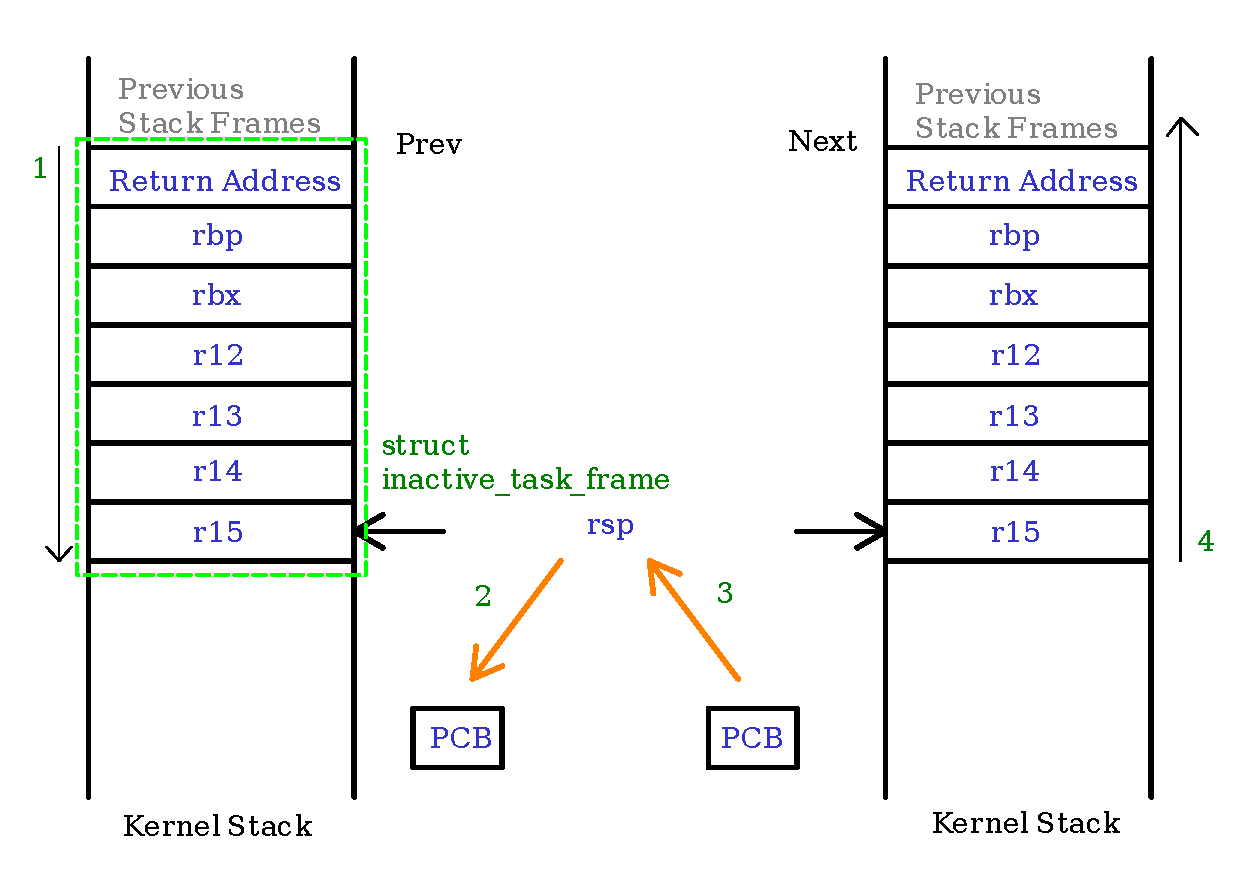
\includegraphics[width=\textwidth]{img/switch_to.pdf}
	\caption{\label{fig:switch_to} 进程切换中的内核栈切换}
\end{figure}


\begin{qbox}{\lstinline{struct thread_info} 与 PCB是什么关系呢?}
	\lstinline{struct task_struct}是进程控制块,
	而 \lstinline{struct thread_info} 存放的也是进程信息,
	只是这些信息更接近底层硬件,且需要能在汇编代码中直接使用.
	\lstinline{struct thread_info} 的大小被控制在一个cache行内,这是由于这些底层信息需要被频繁查看,cache miss会造成较大影响.
	为了尽量利用空间,所有信息都按位编码在其中.
	例如,上文提到的“内核使用了浮点或向量运算而需要加载原来的FPU状态”,
	就存储在 \lstinline{thread_info} 的第 \lstinline{TIF_NEED_FPU_LOAD}
	\footnote{\lstinline{arch/x86/include/asm/thread_info.h} 中定义的宏.} 位.

	\lstinline{struct thread_info} 在更早的Linux版本中位于进程的内核栈的起始位置
	\cite{bovet2005understanding},
	可能造成一些疑惑.
	现在的x86 Linux内核默认把 \lstinline{struct thread_info} 放入
	\lstinline{struct task_struct},
	与PCB的其他成员处于类似的地位.
	\footnote{见 \url{https://lore.kernel.org/all/cover.1473801993.git.luto@kernel.org/}}
	\footnote{见 \url{https://lore.kernel.org/all/a50eab40abeaec9cb9a9e3cbdeafd32190206654.1473801993.git.luto@kernel.org}}
\end{qbox}

\subsection{标识符、进程控制块的链表} \label{process identifiers}
识别进程的方式有很多,首先,指向\lstinline{task_struct} 的指针就可以唯一地确定一个进程.
每一个进程还有编号,记录在 \lstinline{pid_t pid;} 域中.
每一个进程按照创建顺序编号,每一个进程的这个 \lstinline{pid} 域都不相同.
由于 \ref{creating task} 中会介绍的原因,
操作系统的使用者会期望某些调度单元的PID相同.
这是通过 \lstinline{task_struct} 的 \lstinline{pid_t tgid} (thread group id) 域来实现的.
不同的 \lstinline{task_struct} 的 \lstinline{pid} 不能相同,
\lstinline{tgid} 却可能相同.
用户所得到的PID实际上是 \lstinline{task_struct} 中的 \lstinline{tgid}
而不是 \lstinline{pid}.

进程的产生和销毁是动态的,这意味着进程控制块也需要动态分配,
所有分配出来的进程控制块的地址都要通过某种方式留存起来,以供访问.
Linux内核记录多个进程控制块的方式之一是建立包含进程控制块的双向链表.
链表有多种实现,节点互相链接,每个节点指向一个表内的实体的方式为“非侵入式(non-intrusive)”的链表,
实体中包含所需的链表指针的链表为“侵入式”链表.
如果比较访问下一个节点数据的性能,非侵入式链表比侵入式链表性能更好,
因为非侵入式的链表少一次解引用的访存操作.
另外,寻找链表首尾元素和双向遍历的功能也比较重要,
因此内核使用的链表是侵入式的双向链表.

如图~\ref{fig:task_list}所示,
\lstinline{struct list_head} 作为链表的节点,
有 \lstinline{prev} 和 \lstinline{next} 两个指针,
分别指向前一个节点和后一个节点.
链表中的元素通过成员中的 \lstinline{struct list_head} 就可以互相链接.

除了构成全系统的进程表的 \lstinline{struct list_head tasks},
\lstinline{task_struct} 中还包括其他的 \lstinline{list_head},
用于记录与该进程相关的其他进程.
比如,记录树形的父子进程的关系(见\ref{creating task}),
就是通过 \lstinline{struct list_head children}
和 \lstinline{struct list_head sibling}这两个链表实现的.
显然,类似于树的Leftmost child, right sibling表示法\cite{sedgewick2001algorithms},
\lstinline{children} 指向的就应该是某个子进程的 \lstinline{sibling} 成员,
而不是 \lstinline{children} 成员.
以创建进程为例,需要把当前进程的 \lstinline{sibling} 成员,
插入到父进程的 \lstinline{children} 所指的链表尾部:
\begin{lstlisting}[language=C]
/*
 * kernel/fork.c
 * copy_process()
 */
list_add_tail(&p->sibling, &p->real_parent->children);
\end{lstlisting}
\begin{figure}[]
	\centering
	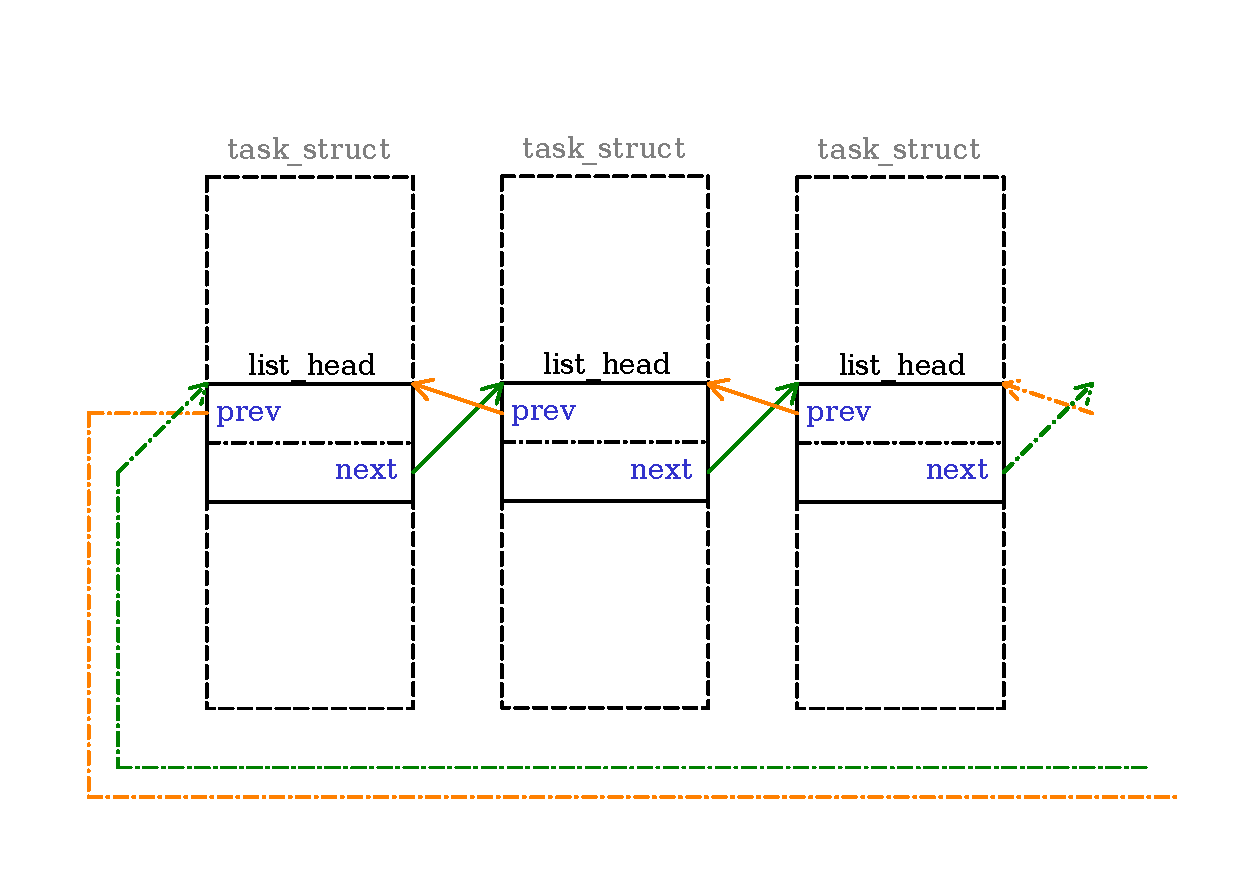
\includegraphics[width=\textwidth]{img/intrusive_list.pdf}
	\caption{\label{fig:task_list} 侵入式双向链表}
\end{figure}

进程控制块还需要通过PID快速获取,这是通过散列表实现的,这里不详细介绍.

\subsubsection{其他信息}
进程控制块中还包括这些方面的相关信息:内存管理、打开的文件、文件系统、调度器、统计数据等.

\begin{itemize}
	\item\textit{内存管理:} 进程的虚拟地址空间信息,\textbf{页表}(将在 TODO 中介绍)
	\item \textit{文件:} 内核需要维护进程\textbf{打开的文件的表},以记录该进程读写文件的状态.
	\item \textit{文件系统:} 记录进程的\textbf{工作目录}和,操作文件所用的\textbf{权限}等.
	\item \textit{调度:}进程所属的\textbf{调度类型},进程的\textbf{优先级}等. (将在TODO中介绍)
	\item \textit{异常处理/进程通信:}进程等待接收的\textbf{信号},信号的屏蔽情况,\textbf{信号处理程序}的地址.
\end{itemize}

\subsubsection{进程和线程的创建} \label{creating task}

\begin{qbox}{内核中线程和进程的区别是什么?}
	前文我们一直以“进程”来描述Linux内核调度的单位.
	即使代码中出现了 \lstinline{thread} 的字样,
	我们仍用“进程”指代.
	实际上,Linux一直使用task来称呼调度的单位,
	只是在和CPU线程有关的地方使用了thread的说法.
	下文将涉及Linux内核中线程和进程的区别.
\end{qbox}

内核中第一个进程是在启动时创建的,PID为0,名为空闲进程(the idle thread),
内核中有一个 \lstinline{struct task_struct init_task}
作为静态的全局变量,在启动时各个成员被赋上相对固定的初始值.
在内核的启动过程中,空闲进程进行一定的初始化,
然后就创建PID为1的进程(the init process),
进一步初始化,最后载入init程序\cite{bovet2005understanding}
(Arch Linux中即为systemd).

除了第一个进程是静态分配,从零开始初始化的,
其余进程的创建都是通过创建已有进程的拷贝来完成的.
这种模式可以追溯到Unix之前的系统,
但是Unix系统采用这种 \lstinline{fork} 的进程创建方式主要是因为实现上较为简单.\cite{ritchie1979evolution}
Linux 跟随Unix的设计思路,提供类似的接口,但又有所不同.

用于复制进程从而创建进程的多种系统调用最终都会使用 内核中的同一段代码,
只是调用时的参数不同,父进程和子进程共享的内容就不同.
可以共享的内容例如:
\begin{itemize}
	\item 父进程(是否使用与被复制的进程相同的父进程);
	\item 虚拟内存空间;
	\item 打开的文件;
	\item 文件系统信息(工作目录、根目录等);
	\item 进程组信息(是否在一个组,tgid);
	\item 信号处理程序,信号屏蔽状态;
	\item 其他资源如I/O.
\end{itemize}
有些资源如栈是不能被共享的,每一个进程需要在自己的栈上运行.
Linux内核有在进程间共享资源的能力,是因为进程控制块中的某些信息并不直接存储在进程控制块中,
而是单独存在,进程控制块中只记录指针.\cite{silberschatz2021operating}

按照这种方式,只要使用不冲突的参数组合,Linux内核就可以创建多种进程,
有些可以被看作“进程”,有些可以可以被看作“线程”,
还有介于“进程”和“线程”之间的,
Linux全部把他们当作调度的单位.
具体的线程模型(不同线程直接共享哪些数据,如何进行控制等)
一般是由 POSIX标准\cite{pthread}定义的,
实现POSIX Thread (pthread)的程序库提供创建线程的函数,
用合适的参数通过系统调用创建符合标准的线程.

\begin{readsrcbox}{进程创建}
	\lstinline{struct task_struct init_task} 的定义在 \lstinline{init/init_task.c}
	中.
	创建进程的函数主要在 \lstinline{kernel/fork.c},
	其调用关系为:
	\begin{itemize}
		\item \lstinline{kernel_clone}
		      \begin{itemize}
			      \item \lstinline{copy_process}
			            \begin{itemize}
				            \item \lstinline{copy_thread} \\
				                  (架构相关,在\lstinline{arch/x86/kernel/process.c})
			            \end{itemize}
		      \end{itemize}
	\end{itemize}
\end{readsrcbox}
